\documentclass{beamer}

\usepackage{lmodern}
\usepackage{tgpagella}
\usepackage{amsmath}
\usepackage{bm}
\usepackage{graphicx} % Required for including images
\usepackage{tikz}
\usepackage{silence}

\usepackage[backend=bibtex]{biblatex}
% Filter warnings issued by package biblatex starting with "Patching footnotes
% failed"
\WarningFilter{biblatex}{Patching footnotes failed}

% Required for specifying captions to tables and figures
\usepackage{amsfonts, amsmath, amsthm, amssymb}
\usepackage[most]{tcolorbox}

\usetikzlibrary{arrows,arrows.meta,automata,calc}
\bibliography{presentation}

% Math shorthands
\newcommand{\paren}[1]{\left(#1\right)}
\newcommand{\Z}{\mathbb{Z}}
\newcommand{\N}{\mathbb{N}}
\newcommand{\Q}{\mathbb{Q}}
\newcommand{\ch}[1]{\mathbf{#1}}
\newcommand{\A}{\mathcal{A}}
\newcommand{\gp}{\mathcal{G}}
\newcommand{\res}[2]{{{#1}_{\ch{#2}}}}
\newcommand{\F}{\mathcal{F}}
\newcommand{\M}{\mathcal{M}}
\newcommand{\bin}{\pmb{\bm{2}}}
\newcommand{\orb}{\mathbf{orb}}
\newcommand{\R}{\mathbf{R}}
\newcommand{\f}[1]{\overline{#1}}
\newcommand{\rej}{\mathbf{rej}}

\newcommand{\codeurl}{\texttt{https://github.com/tim-becker/thesis-code}}

\tikzset{%
        ->,
        auto,
        shorten > = 2pt,
        node distance=2.5cm
}
\tikzstyle{every state}=[
    draw = black,
    style = thick,
    fill = white,
    line width = 1pt,
    minimum size = 5mm
]
\tikzstyle{every edge}=[
    style = thick,
    draw = black,
    line width=1pt,
]

\usetheme{Boadilla}

\title[Abelian Automaton Groups]
{Representations and Complexity of Abelian Automaton Groups}
\author[Tim Becker]{Tim Becker\texorpdfstring{\\{\small
            Advised by: Klaus Sutner}}{}}
\institute{Carnegie Mellon University}
\date{May 9, 2018}

\newsavebox{\grigorchuk}
\savebox{\grigorchuk}{
    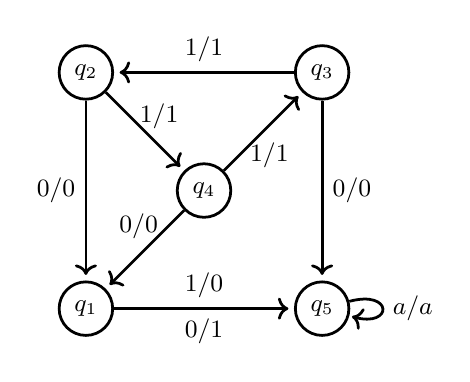
\begin{tikzpicture}[node distance=3.0cm]
        \node[state] (1) {\small $q_1$};
        \node[state] (2) [above of=1] {\small $q_2$};
        \node[state] (3) [right of=2] {\small $q_3$};
        \node[state] (4) at ($(1)!0.5!(3)$) {\small $q_4$};
        \node[state] (5) [right of=1] {\small $q_5$};
      \path
      (1)
      edge node{\small $1/0$} node[swap]{\small $0/1$} (5)
      (2)
      edge node[left]{\small $0/0$} (1)
      edge node[right, pos=0.3]{\small $1/1$} (4)
      (4)
      edge node[left, pos=0.2]{\small $0/0$} (1)
      edge node[right, pos=0.2]{\small $1/1$} (3)
      (3)
      edge node[above]{\small $1/1$}  (2)
      edge node[right]{\small $0/0$}  (5)
      (5)
      edge[loop right=45] node{\small $a/a$} (5)
      ;
    \end{tikzpicture}
}

\newsavebox{\ccc}
\savebox{\ccc}{
    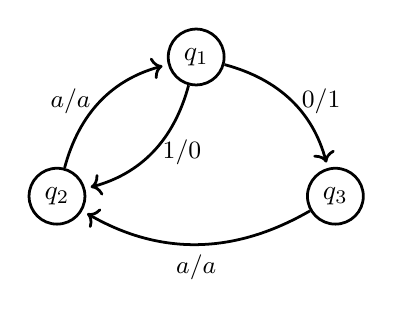
\begin{tikzpicture}
        \node[state] (1) {$q_1$};
        \node[state] (2) [below left of = 1] {$q_2$};
        \node[state] (3) [below right of = 1] {$q_3$};
        \path
        (1) edge[bend left, right]
        node {\small $1/0$} (2)
        (1) edge[bend left, right]
        node {\small $0/1$} (3)
        (2) edge[bend left, left]
        node {\small $a/a$} (1)
        (3) edge[bend left]
        node {\small $a/a$} (2)
        ;
    \end{tikzpicture}
}

\begin{document}

\AtBeginSection[] {
  \begin{frame}
    \frametitle{Table of Contents}
    \tableofcontents[currentsection]
  \end{frame}
}

\begin{frame}
    \titlepage
\end{frame}

\section{Background}

\begin{frame}
\frametitle{Flipping Pebbles}
\begin{center}
    
\includegraphics[scale=.1]{./pebbles-1}
\end{center}

\begin{center}
  {\LARGE\textbf{$\Downarrow$}}
\end{center}

\begin{center}
    
\includegraphics[scale=.1]{./pebbles-2}
\end{center}

\vspace{.5cm}

{\bf \emph{Rule:}}
Given a row of pebbles, white on one side, blue on the other.  Flip the first
pebble.  If it was white, skip the next two pebbles; otherwise, skip just one
pebble.  Keep flipping till you fall off the end.

\end{frame}

\begin{frame}
\frametitle{}
\begin{center}
  \includegraphics[scale=0.025]{pebbles-orbit}
\end{center}
\end{frame}

\begin{frame}
    \frametitle{Invertible Transducers}
    The previous game is described by a deterministic finite state transducer
    with invertible output functions.
    \begin{center}
        \usebox{\ccc}
    \end{center}
\end{frame}

\begin{frame}
    \frametitle{Automaton Groups}
    \begin{itemize}
            \item<1-> States induce a length preserving invertible function on
                binary strings.
            \item<2-> These functions form a group under composition, called an
                \alert{automaton group}.
            \item<3-> These have been useful for some recent results in group
                theory.
    \end{itemize}
    \pause
    \pause
    \pause
    \begin{center}
        \usebox{\grigorchuk}
    \end{center}
\end{frame}

\begin{frame}
    \frametitle{Terminology and Notation}
    \begin{itemize}
        \item<1-> $\bin = \{0, 1\}$ is the binary alphabet.
        \item<2-> $\A$ is an invertible transducer.
        \item<3-> $\A^{-1}$ is the inverse machine, formed by flipping the edge
            labels:
            \begin{align*}
                q_i \xrightarrow{\ch{a} / \ch{b}} q_j
                && \text{becomes} &&
                q_i^{-1} \xrightarrow{\ch{b} / \ch{a}} q_j^{-1}.
            \end{align*}
        \item<4-> $\gp(\A)$ is the group formed by arbitrary compositions of
            transductions from $\A$ and $\A^{-1}$.
        \item<5-> An element of $\gp(\A)$ is \alert{even} if it copies the
            first input bit, and \alert{odd} if it flips it.
    \end{itemize}
\end{frame}

\begin{frame}
    \frametitle{Residuals}
    Any $f \in \gp(\A)$ is a word over the states of $\A$:
    \[
        f = q_{i_1}^{d_1} \,\, q_{i_2}^{d_2}  \cdots q_{i_n}^{d_n},
    \]
    where each $d_i \in \{-1, 1\}$.
    \pause

    Hence $f$ can be seen as a state in the product automaton
    \[
        \mathcal P = \A^{d_1} \times \A^{d_2} \times \cdots \times \A^{d_n}.
    \]
    \pause
    For $\ch{a} \in \bin$, then $\res{f}{a}$ is the \alert{$\ch{a}$-residual}
    of $f$: the state in $\mathcal P$ which $f$ transitions to on input
    letter $\ch{a}$.
    \begin{center}
        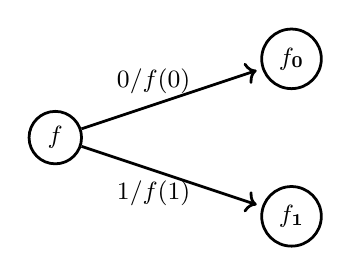
\begin{tikzpicture}
            \node[state] (f) at (0, 0) {\small $f$};
            \node[state] (f0) at (3, 1) {\small $\res{f}{0}$};
            \node[state] (f1) at (3, -1) {\small $\res{f}{1}$};
            \path
                (f) edge node[above, pos=0.4] {\small $0 / f(0)$} (f0)
                (f) edge node[below, pos=0.4] {\small $1 / f(1)$} (f1)
                ;
        \end{tikzpicture}
    \end{center}
\end{frame}

\begin{frame}
    \frametitle{Abelian Automata}
    We will focus on machines $\A$ where $\gp(\A)$ is abelian, i.e.\ where
    all transductions commute.
    \pause
    \begin{center}
        \usebox{\ccc}
    \end{center}
    \pause
    As functions over binary strings, we have $q_i q_j = q_j q_i$ for $i,j \in
    \{1, 2, 3\}$. Hence $\gp(\A)$ is abelian.
\end{frame}

\begin{frame}
    \frametitle{Gap Lemma}
    Define the \alert{gap value} of any $f \in \gp(\A)$ as
    $\gamma_{f} = \res{f}{0} \res{f}{1}^{-1}$.
    \pause

    \vspace{.5cm}
    {\bf \emph{Gap Lemma:}} $\gp(\A)$ is abelian if and only if every odd element
    has the same gap value and every even element has gap value equal to
    the identity function.

\end{frame}
\begin{frame}
    \frametitle{Gap Lemma}
    Thus in an abelian automaton, there is a global gap value $\gamma$ such
    that for all odd $f \in \gp(\A)$, $\res{f}{0} = \gamma \res{f}{1}$. Also if
    $g$ is even, then $\res{g}{0} = \res{g}{1}$.

    \vspace{.5cm}
    \begin{center}
        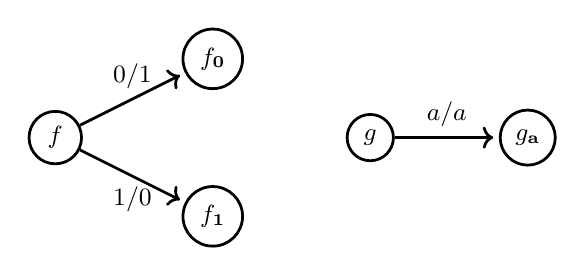
\begin{tikzpicture}
            \node[state] (f) at (0, 0) {\small $f$};
            \node[state] (f0) at (2, 1) {\small $\res{f}{0}$};
            \node[state] (f1) at (2, -1) {\small $\res{f}{1}$};
            \node[state] (g) at (4, 0) {\small $g$};
            \node[state] (ga) at (6, 0) {\small $\res{g}{a}$};
            \path
            (f)
            edge node[above] {\small $0/1$} (f0)
            edge node[below] {\small $1/0$} (f1)
            (g)
            edge node[above] {\small $a/a$} (ga)
            ;
        \end{tikzpicture}
    \end{center}
\end{frame}

\section{Classifying Orbit Complexity}

\begin{frame}
    \frametitle{Orbits}
    The \alert{orbit} of a string $\ch{x} \in \bin^k$ under $f$ is
    \[
        \{\ch{y} \in \bin^k \mid \exists t \in \Z \text{ such that }
        f^t(\ch{x})\}.
    \]
    \pause
    The \alert{orbit language} of $f$ is
    \[
        \orb(f) = \{\ch{x}{:}{\ch{y} \mid \exists t \in \Z
                \text{ such that } f^t (\ch{x}) = \ch{y}}\}
    \]
    where $\ch{x} {:} \ch{y}$ is the convolution two words $\ch{x}, \ch{y}
    \in \bin^k$:
    \[
        \ch{x} {:} \ch{y} = \begin{tabular}{|c|c|c|c|}
            \hline
            $\ch{x_1}$ & $\ch{x_2}$ & $\ldots$ & $\ch{x_k}$\\
            \hline
            $\ch{y_1}$ & $\ch{y_2}$ & $\ldots$ & $\ch{y_k}$\\
            \hline
        \end{tabular} \in (\bin \times \bin)^k.
    \]
    \pause

    \vspace{.5cm}
    {\bf \emph{Orbit Problem:}} Given $f \in \gp(\A)$ and $\ch{x}, \ch{y}
    \in \bin^k$, is $\ch{x}{:}\ch{y} \in \orb(f)$.
\end{frame}

\begin{frame}
    \frametitle{Orbit Complexity}
    The orbit problem is clearly decidable: the orbit of a string
    $\ch{x}$ is finite (bounded above by $2^{|\ch{x}|}$).
    \pause

    \vspace{.3cm}
    Also, this bound is tight. The adding machine achieves it.
    \begin{center}
        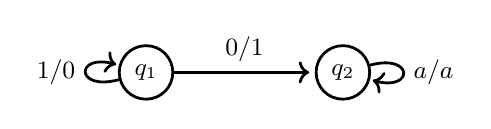
\begin{tikzpicture}
            \node[state] (1) {\small $q_1$};
            \node[state, right of=1] (2) {\small $q_2$};
            \path
            (1)
            edge[loop left=45] node[left] {\small {$1 / 0$}} (1)
            edge node[above] {\small {$0 / 1$}} (2)
            (2)
            edge[loop right=45] node[right] {\small {$a / a$}} (2)
            ;
        \end{tikzpicture}
    \end{center}
\end{frame}

\begin{frame}
    \frametitle{Poll}
    \begin{center}
        \scalebox{.8}{\usebox{\ccc}}
    \end{center}
    For state $q_1$ and for $\ch{x},\ch{y} \in \bin^{1,000,000}$, how quickly
    can we solve the orbit problem?
    \begin{itemize}
        \item seconds?
        \item minutes?
        \item days?
        \item years?
        \item longer?
    \end{itemize}
\end{frame}

\begin{frame}
    \frametitle{Rationality}
    {\bf \emph{Goal:}} Determine when $\orb(f)$ is regular.
    \pause

    Brzozowski: it suffices to show $\orb(f)$ has finitely many quotients.
    \pause

    We can describe the quotients by adding a translation function.  Let
    \[
        \R(f, g) = \{\ch{x}:\ch{y} \mid \exists t \in \Z
        \text{ such that } g(f^t(\ch{x})) = \ch{y}\}
    \]
    Then $\R$ is closed under quotients: if $f, g \in \gp(\A)$ and $\ch{b} =
    g(\ch{a})$, then
    \begin{align*}
        (\ch{a} {:} \ch{b})^{-1} \R(f, g) &=
        \begin{cases}
            \R(\res{f}{a}, \res{g}{a}) & \text{if $f$ is even,}\\
            \R(\res{f^2}{a}, \res{g}{a}) & \text{if $f$ is odd.}
        \end{cases}\\
        (\ch{a} {:} \f{\ch{b}})^{-1} \R(f, g) &=
        \begin{cases}
            \emptyset & \text{if $f$ is even,}\\
            \R(\res{f^2}{a}, \res{f}{a}\res{g}{\f{a}}) &
            \text{if $f$ is odd.}
        \end{cases}
    \end{align*}
\end{frame}

\begin{frame}
    \frametitle{Abelian Orbits}
    In abelian automaton groups, there are finitely many quotients if and only
    if there are finitely many first components (because $\gp(\A)$ is
    ``contracting'').
    \pause

    \vspace{.5cm}
    Further, the first components are determined by the simple map
    \[
        \varphi(f) = \begin{cases}
            \res{f}{a} & \text{if $f$ is even,}\\
            \res{f^2}{a} & \text{if $f$ is odd.}
        \end{cases}
    \]
    \vspace{.5cm}
    Thus we must only determine if $\varphi^*(f)$ is finite.
\end{frame}

\begin{frame}
    \frametitle{Algebra to the Rescue}
    We can associate to $\gp(\A)$ an algebraic number $\alpha$ and an embedding
    $\Psi: \gp(\A) \rightarrow \Q(\alpha)$ such that if $f$ is even, then
    $\Psi(\res{f}{a}) = \alpha\Psi(f)$.
    \pause

    \vspace{.3cm}
    Under $\Psi$, $\varphi$ has the simple form
    \[
        \Psi(\varphi(f)) = \begin{cases}
            \alpha \Psi(f) & \text{if $f$ is even,}\\
            2\alpha \Psi(f) & \text{if $f$ is odd.}
        \end{cases}
    \]
    \pause
    Using a few more tricks, the following theorem follows:\\
    \vspace{.3cm}
    {\bf \emph{Theorem:}} $\orb(f)$ is rational if and only if some power of
    $\alpha$ is rational.
\end{frame}

\section{Computing the number field}

\begin{frame}
    \frametitle{Goal}
    Embed $\gp(\A)$ in some algebraic object, while preserving residuation
    structure in a useful way.
\end{frame}

\begin{frame}
    \frametitle{System of Equations}
    Want to find a map $\Psi : \gp(\A) \rightarrow \Q(\alpha)$ where
    residuation is given by
    \[
        \Psi(\res{f}{a}) = \begin{cases}
            \alpha \Psi(f) & \text{if $f$ is even,}\\
            \alpha \Psi(f) + (-1)^a & \text{if $f$ is odd.}
        \end{cases}
    \]

    \begin{columns}
    \begin{column}{0.33\textwidth}
        \begin{center}
            \scalebox{.8}{\usebox{\ccc}}
        \end{center}
    \end{column}
    \begin{column}{0.33\textwidth}
        \LARGE
        \begin{align*}
            \implies
        \end{align*}
    \end{column}
    \begin{column}{0.33\textwidth}
        \begin{align*}
            z x_1 + 1 &= x_3\\
            z x_1 - 1 &= x_2\\
            z x_3 &= x_2\\
            z x_2 &= x_1
        \end{align*}
    \end{column}
    \end{columns}
    \pause
    \vspace{.5cm}

    Solving this system equations will produce suitable values for $\alpha$,
    $\Psi(q_1), \ldots, \Psi(q_n)$.
\end{frame}

\begin{frame}
    \frametitle{How to solve it}
    This system can interpreted as an ideal of a polynomial ring with unknowns
    for $\alpha$ and for each state in $\A$. Computing a Gr\"obner basis of
    this ideal gives an easy way to enumerate the solutions.
    \pause

    \vspace{.5cm}
    In general, Gr\"obner bases are expensive to compute (EXPSPACE-complete),
    but because our equations are ``nearly linear'', we can compute a Gr\"obner
    basis in time $O(n^6)$.
\end{frame}

\begin{frame}
    \frametitle{Solution}
    $\alpha$ has minimal polynomial $\chi(z) = z^2 + z + 1/2$.
    \vspace{.5cm}
    \begin{center}
    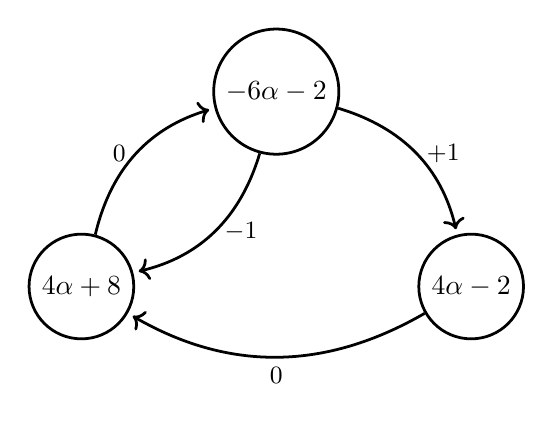
\begin{tikzpicture}[node distance = 3.5cm]
        \node[state] (1) {$-6\alpha - 2$};
        \node[state] (2) [below left of = 1] {$4 \alpha + 8$};
        \node[state] (3) [below right of = 1] {$4 \alpha - 2$};
        \path
        (1) edge[bend left, right]
        node {\small $-1$} (2)
        (1) edge[bend left, right]
        node {\small $+1$} (3)
        (2) edge[bend left, left]
        node {\small $0$} (1)
        (3) edge[bend left]
        node {\small $0$} (2)
        ;
    \end{tikzpicture}
    \end{center}
    \tiny{(The embeddings shown are scaled by 5 for simplicity)}
\end{frame}

\begin{frame}
    \frametitle{Summary}
    By computing an algebraic number associated to $\gp(\A)$, we can check if
    $\A$ has a rational orbit relation in time $O(n^6)$.
    \pause

    \vspace{.5cm}
    We expect this algebraic tool to assist in other computational problems
    arising in these automata.

    \pause
    \vspace{.5cm}
    All algorithms discussed were implemented in Sage; code is available at
    \[
        \codeurl.
    \]
\end{frame}

\begin{frame}
    \frametitle{Acknowledgements}

    Klaus Sutner for advising this project.

    \vspace{.8cm}

    Evan Bergeron for many helpful conversations.
\end{frame}

\begin{frame}
    \frametitle{Questions?}
\end{frame}

\end{document}
